\documentclass[12pt]{article}
\usepackage[utf8]{inputenc}
\usepackage{indentfirst}
\usepackage{graphicx}
\usepackage{hyperref}
\hypersetup{
    colorlinks,
    citecolor=black,
    filecolor=black,
    linkcolor=red,
    urlcolor=black,
}
\usepackage[export]{adjustbox}
\usepackage[super]{nth}
\usepackage{caption}

\title{\textbf{Internship Report} \\ Val d'Oise Departmental Council}
\author{Cinquanta Octave \\ CY Tech Student}
\date{July 22, 2020}

\begin{document}

\begin{figure}[t]
    \centering
    
\includegraphics[width=0.20\textwidth,right]{Cergy Ygrec Logo.jpg}
    \label{Logo}
\end{figure}

\maketitle

\section{Dedication}

I wish to dedicate my work to my internship supervisor and friend Nicolas Maître, who was the one to present me with an opportunity to do my first-year internship at the Departmental Council. This internship wouldn't have been possible without his help and he has done a great job at being my supervisor during its duration.

\section{Acknowledgement}

I wish to acknowledge the help I received when writing this report. I wish to thank my parents for the proofreading of this document, especially my mother for the orthographic check and my father for the semantic check. I also wish to thank my supervisor once again and his colleagues for the information they gave me about the Council.

\section{Executive Summary}

During this report, I will first introduce the Council I worked at, meaning its history and the way it operates. I will then explain its organizational structure and provide a chart for the specific branch I worked in. Next I will present the directorate in which my internship was done, as well as give the specifics if the internship. Then will I describe my supervisor's work, and the different tasks that were given to me. The next section includes a reflection on three specific days of the internship where I learned useful things and gained precious company experience. Afterwards, I will proceed to executing two analysis and use them to write a conclusion to my internship and a recommendation to the Council.

\tableofcontents
\listoffigures

\section{Overview of the Organization}

The Val d'Oise department was created during the 1964 Paris Region reorganization. It used to be part of the old region Seine-et-Oise that was dismantled by the law of the \nth{10} of July 1964. In 2014, the number of cantons in the department was reduced from 39 to 21, with each canton electing 2 members of the Council. Therefore from 2015 onward the Council has 42 members who elect their own president and vice-presidents. Before 2015, its name was also different, as it would be called then the Val d'Oise General Council. \\
Like other departmental councils, it has different missions to manage given to him by the government. Those include welfare, the management of roads, transports, education, culture, local development, tourism and even housing. Because of the quantity and diversity of these tasks, the Council is composed of many sections and subsections of employees, each one of them being given different specific tasks. \\
As a common law community, the Council doesn't have any competitor, although it can be compared to another community, which is the Île-de-France Regional Council, whose missions are different. The government can also choose to redistribute certain missions from the Departmental to the Regional Council as it happened in 2015 with the matter of public transportation.

\clearpage
\section{Organizational Structure}

\begin{figure}
    \centering
    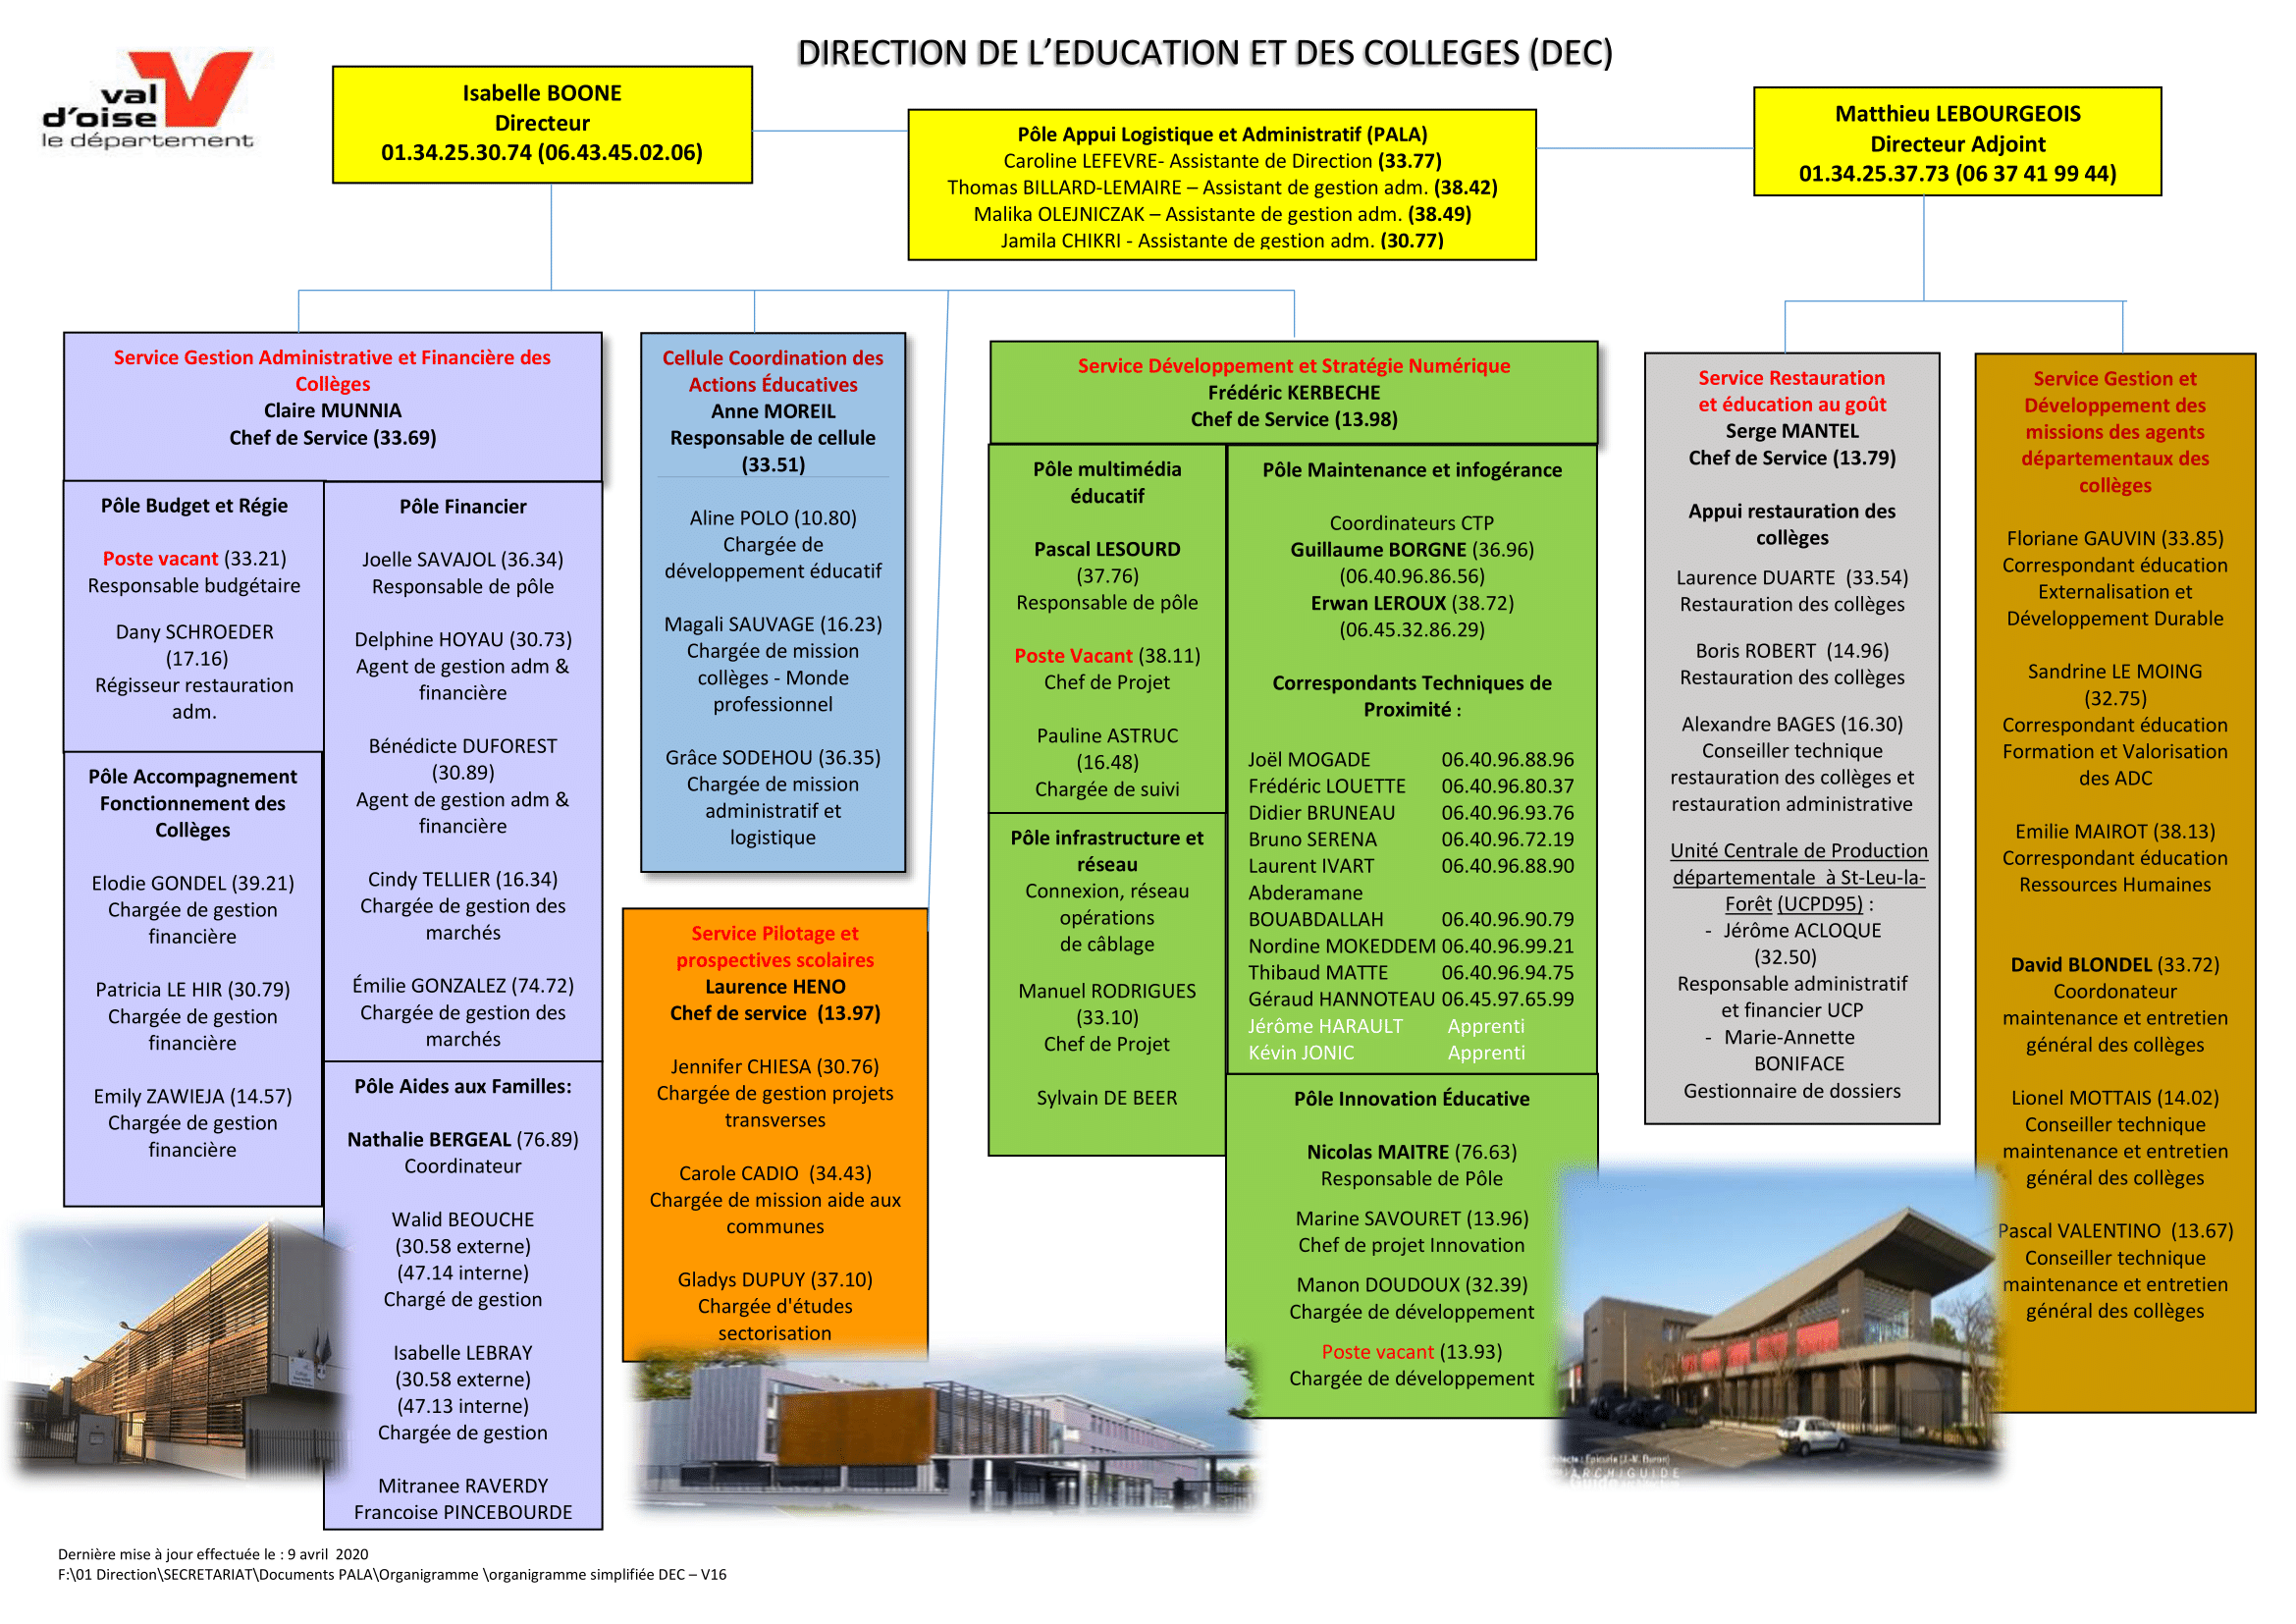
\includegraphics[width=1.5\textwidth,center]{Organigramme.png}
    \captionsetup{justification=centering}
    \caption{Organizational Chart of the Education and Middle Schools Directorate}
    \label{Orga}
\end{figure}

The number of employees in the Departmental Council is more than 2000 people. \\
The main offices of the Departmental Council are located in Cergy at 2 avenue du Parc. On site there is twelve different buildings labeled from A to L, and different floors of those buildings are assigned to the branches and directorates of the Council. Those branches include : \\
- the General Services Direction made of the Legal Affairs Directorate, the External Communication Directorate, the Intern Communication and Information Management Directorate, the Innovation Mission Directorate and the Human Resources Directorate. \\
- the Solidarity Direction made of the Childhood Directorate, the Disabled Persons Directorate, the Old Persons Directorate, the Prevention and Health Directorate and the Social Life Directorate \\
- the Administrative Direction made of the Public Procurement and Resources Directorate, the Archives Directorate, the Finances Directorate, the Heritage Management Directorate and the Information Technology Directorate \\
- the Territory Development Direction made of the Roads Directorate, the Environment and Sustainable Development Directorate, the Grand Eastern Paris Directorate, the Territory and Housing Directorate and the Transports Directorate \\
- and the Development Direction made of the Cultural Action Directorate, the Economic and International Attractiveness Directorate, the Education and Middle Schools Directorate, the Grand Western Paris Directorate, the Youth, Prevention and Safety Directorate, the Numerical Planning and Development Mission Directorate and the Sports Mission Directorate. \\
The organizational structure of the Council is quite complicated, as there are many Branches and Directorates, and even more Poles. This complex structure allows for the various responsibilities of the Council to be well distributed amongst the employees.

\clearpage
\section{Plan of the Internship Program}

My internship was done in the Education and Middle Schools Directorate of the Departmental Council. This directorate contains six different offices, each containing their own poles, and an extra pole. Those offices include the Middle Schools' Administrative and Financial Management Office, the School Steering and Foresight Office, the Educational Actions Coordination Cell, the Numerical Development and Strategies Office, the Catering and Taste Education Office and the Middle Schools' Departmental Agents' Missions Management and Development Office. My internship supervisor works in the Numerical Development and Strategies Office and is responsible of the Educational Innovation pole, thus this is where my internship was done. This internship began on the \nth{15} of June and ended on the \nth{15} of July, for a total set duration of a month. The work hours were from 9 in the morning to 5 in the afternoon, with approximately an hour for lunch, resulting in 7 hours of work per day, 5 days per week. At the beginning, because of the COVID-19 pandemic and the deconfinement procedures, only 2 days per week were done at the office, the rest in distance working, and in the end up to 4 days were done on site. 

\section{Training Program}

The goal of the Education and Middle Schools Directorate of the Council is the management of all of the Council's responsibilities concerning education, and in particular of public middle schools in the department, as the management of elementary schools is given to communes and the management of high schools to regional councils. Those responsibilities include the property of public middle schools, meaning the management of their edification, their redevelopment, their extension, their important repairs, their equipment and their operation. The Council can also choose to organize educational, athletic and cultural events in the schools. It must also manage the catering of the middle schools, such as fixing the price for a single meal or fixing the amount of social funds given to families to help pay meals. It also deals with the recruitment of school staff excluding teachers, and delimits the zones in which students should go to the nearest public middle school in its department. The Numerical Development and Strategies Office of this directorate is given the task of managing the different numerical tools used by the middle schools. Those include the use of Internet and networks in general, technical maintenance, the students' educational tablets, etc. The pole in which my internship supervisor works, the Educational Innovation pole, is in charge of finding and establishing new uses of the numerical for education, and the management of the middle school digital work-space, \textit{moncollege.valdoise.fr}, used by teachers, students and parents to access work resources, grades, assignments and information, and allows for easy communication between parents and the school. Such are the responsibilities of the Council branch I worked at. \\
As for me, there was no such thing as a general job or project given to me to complete by the end of the internship, but rather a series of tasks varying in size depending on the actual needs of my supervisor and boss, although the majority of tasks ended up being quite anecdotal except for two of them: the MakeX guide translation and the mBot programming. The other tasks could go from writing a simple email, adding accounts to a database, creating Excel sheets from paperwork to an attempt at making HTML graphs using an AtInternet database and having them update themselves automatically after a change in the database's values. Now for the main tasks. At the beginning of the internship, my supervisor showed me a programmable robot called the "mBot", which worked with Scratch code and as such was used by the department to teach early programming to middle school students and allow them to participate in a robotics competition called MakeX, whose guide I translated as the second major task. The goal of this task was to initiate me with the robot, and as such my supervisor asked me to play a song by AC/DC on the robot. Since it was the first task given to me it ended up being the background task of the internship. This may be one of the cause for the fact that this task was left unsuccessful when the time was up. I ended up mostly focusing on other tasks and didn't finish this one, although it did teach me a number of useful things on Python and Scratch alike. I encountered many hardships during this task, such as difference between xml and mxl files, the potential use of Arduino programming, Scratch music players, having to use Python 2.7 modules and Python 3.6 modules at the same time, etc. I had to take a new look on the problem at each failure and learned from those. My second task was given to me by my supervisor's boss, who was working on the management of the MakeX competition in France, and acquired a guide for the competition that was in English, translated from Chinese. He needed for the guide to be in French so that he could give it to the teachers and the students for them to understand the competition, and so he asked me to translate it. The guide was a 48 pages long pdf filled with technical terms of robotics and many diagrams that I had to first understand myself before making others understand it as well. This task wasn't easy, but because I love English and the work of languages in general, it was quite enjoyable. Those were the two main tasks given to me during my internship.

\section{Reflective Journal Entries}

The two days I will use to write the following reflective journal entry are the \nth{6}, \nth{7} and \nth{8} of July, those days being the Monday, the Tuesday and the Wednesday of my internship's third week. At first, I thought those three days would be relatively uneventful and normal days, and they were, with a few exceptions that make them noteworthy. As usual I would start off by setting up my desk and begin the translation of the MakeX competition guide that I was still working on at the time, and I would also keep trying new approaches for the programming of the mBot. Most of the Monday was spent translating, and in the afternoon, we went to a middle school, Les Touleuses, in Cergy. This school is in fact the biggest public middle school of the department, and it was in the middle of its renovation when we came. My supervisor was given the task of retrieving a short story dispenser that had ceased to function a few days beforehand. Because we had to transport a relatively heavy item, my supervisor was given a trolley, a special cardboard box for the machine's glass panel and the car he was lent was a Citroen C3, for the machine to fit in the car's boot. So, we went to the school, and met with the principal, who talked with us about the ongoing changes in the school and served as our guide and door opener throughout the maze-like corridors of the school. When we reached the school's library, we split the machine in two: my supervisor took the heavy bottom half containing the printer and put in on the trolley to carry it, and I took the glass panel, inserted it in the cardboard box and we then left for the car. Upon arrival we transported the machine to my supervisor's office, where it still stands as of today, waiting for its retrieval by the people in charge of repairing it. On Tuesday, every member of the Numerical Development and Strategies Office was invited to a meal at the nearest Ristorante del Arte, and so was I. It was a casual meeting outside of work used to celebrate the nearing end of the school year, and as such was a pleasant little break. In the afternoon of the Tuesday, as I was fiddling with the mBot, my supervisor's boss came in the office and was looking for help. My supervisor was, like most of the time, quite busy so he asked if I could do him a favor and I obviously accepted. He gave me two equipment delivery statements on which he had scribbled different letters on different objects. He told me that each of the four letters corresponded to a certain middle school and that he wanted me to create an Excel file that simply resumed what object was to be delivered to which middle school and specify the quantity of each item. So, I did, and about five minutes later I sent him the Excel sheet. On Wednesday, because of the COVID-19 procedures, both my supervisor and I were working from our homes, and I was still translating the guide. He then sent me an email from his boss with nine other emails in attachment and asked me to create an Excel Sheet serving as a digest version of all the emails. Those were actually project demands from different middle schools, and the project had the goal of developing Eco-delegates. Eco-delegates are chosen students that engage in various activities to promote sustainable development, and as such the projects revolved around creating and establishing different ecological actions in the schools. I had to summarize the projects by their school, address, teachers involved, number of students involved, actions undertook, etc. and I was done by the end of the day. \\
Those various tasks and events taught me a few things about the sort of work my supervisor's is and about the relationships of colleagues in and out of a work-place.\\
One thing that wasn't always clear in my head was the limits of what my supervisor's work and responsibilities were supposed to be. I knew he was responsible for the management of the middle school digital work-place, and that his job as head of the Educational Innovation pole gave him the responsibilities to manage many numerical issues concerning middle schools. That concept was quite vague and didn't really set as much as a border to delimit his work. And in fact, this concept was the closest thing to describe his work. This work had certain set responsibilities, and other tasks, like the retrieval of the story dispenser, could be given to him at any time, and he has to manage many different things and people, as much as to delay his own main work. This gave his work a more complex structure than what could be guessed from just its title. As my first true experience in a company it gave me many insights that may seem obvious to most experienced people. For instance, the restaurant meal gave me a more jovial yet serious impression of the company. The relationship between its members was professional in every way, yet it looked as though it was also friendly when outside of work, and it was quite a reassuring sight as being colleagues didn't look any different than being fellow students anymore. I also learned from the Excel tasks I had to do that in a company, the more serious and working one is, the more work will be given to them. I am in fact referencing here to my internship supervisor. He is quite the skilled and responsible worker, as any task he is given will be done neatly and rapidly. As such I saw that his boss gives him quite the amount of work, but at the same time is quite close and trustful towards him. This relationship was a healthy one, and as such I thrive to obtain such a relationship towards any future employer and/or employee. \\
Such are the things I was able to observe during those three days, and I am quite sure that they will prove to be useful experience in the near future when I work in a company again.

\section{Work Samples}

\begin{figure}[h]
    \centering
    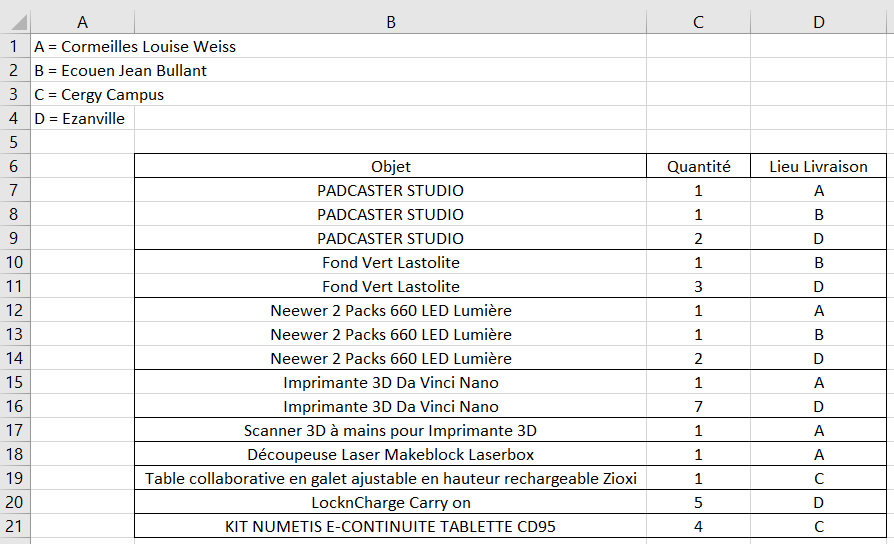
\includegraphics[width=\textwidth]{EASYTIS.png}
    \caption{The aforementioned Excel sheet tasked on Tuesday the \nth{7}}
    \label{sheet}
\end{figure}

\begin{figure}
    \centering
    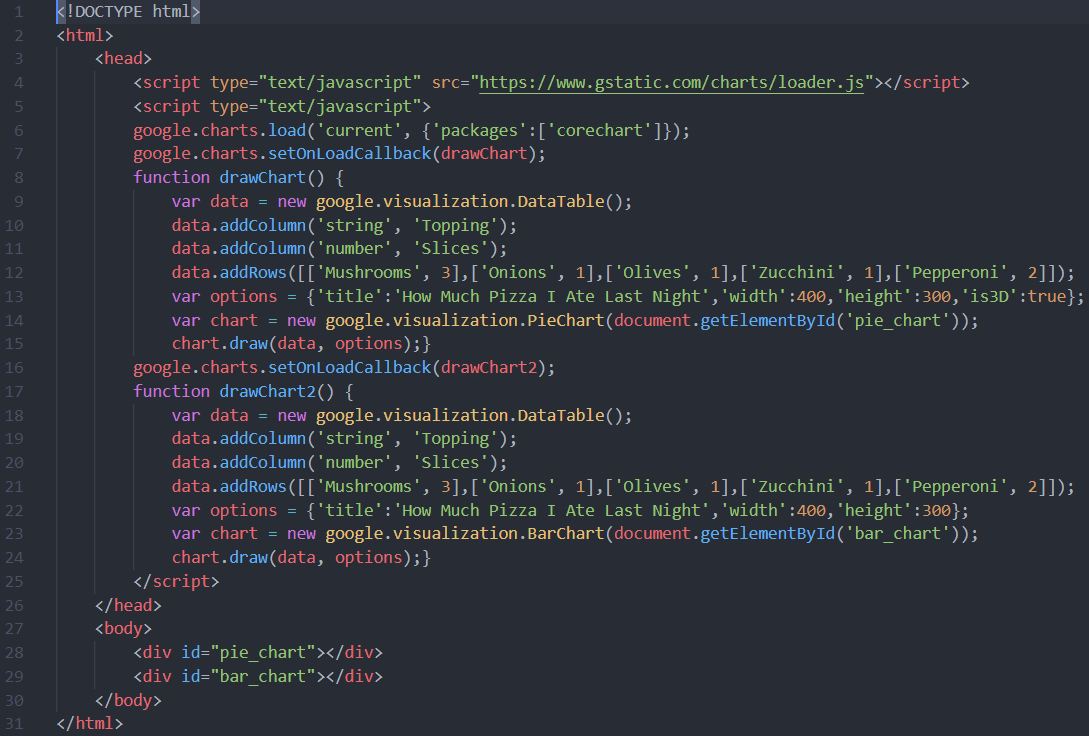
\includegraphics[width=\textwidth]{graph.PNG}
    \caption{An example of code for HTML graphs}
    \label{html graph}
\end{figure}

\begin{figure}
    \centering
    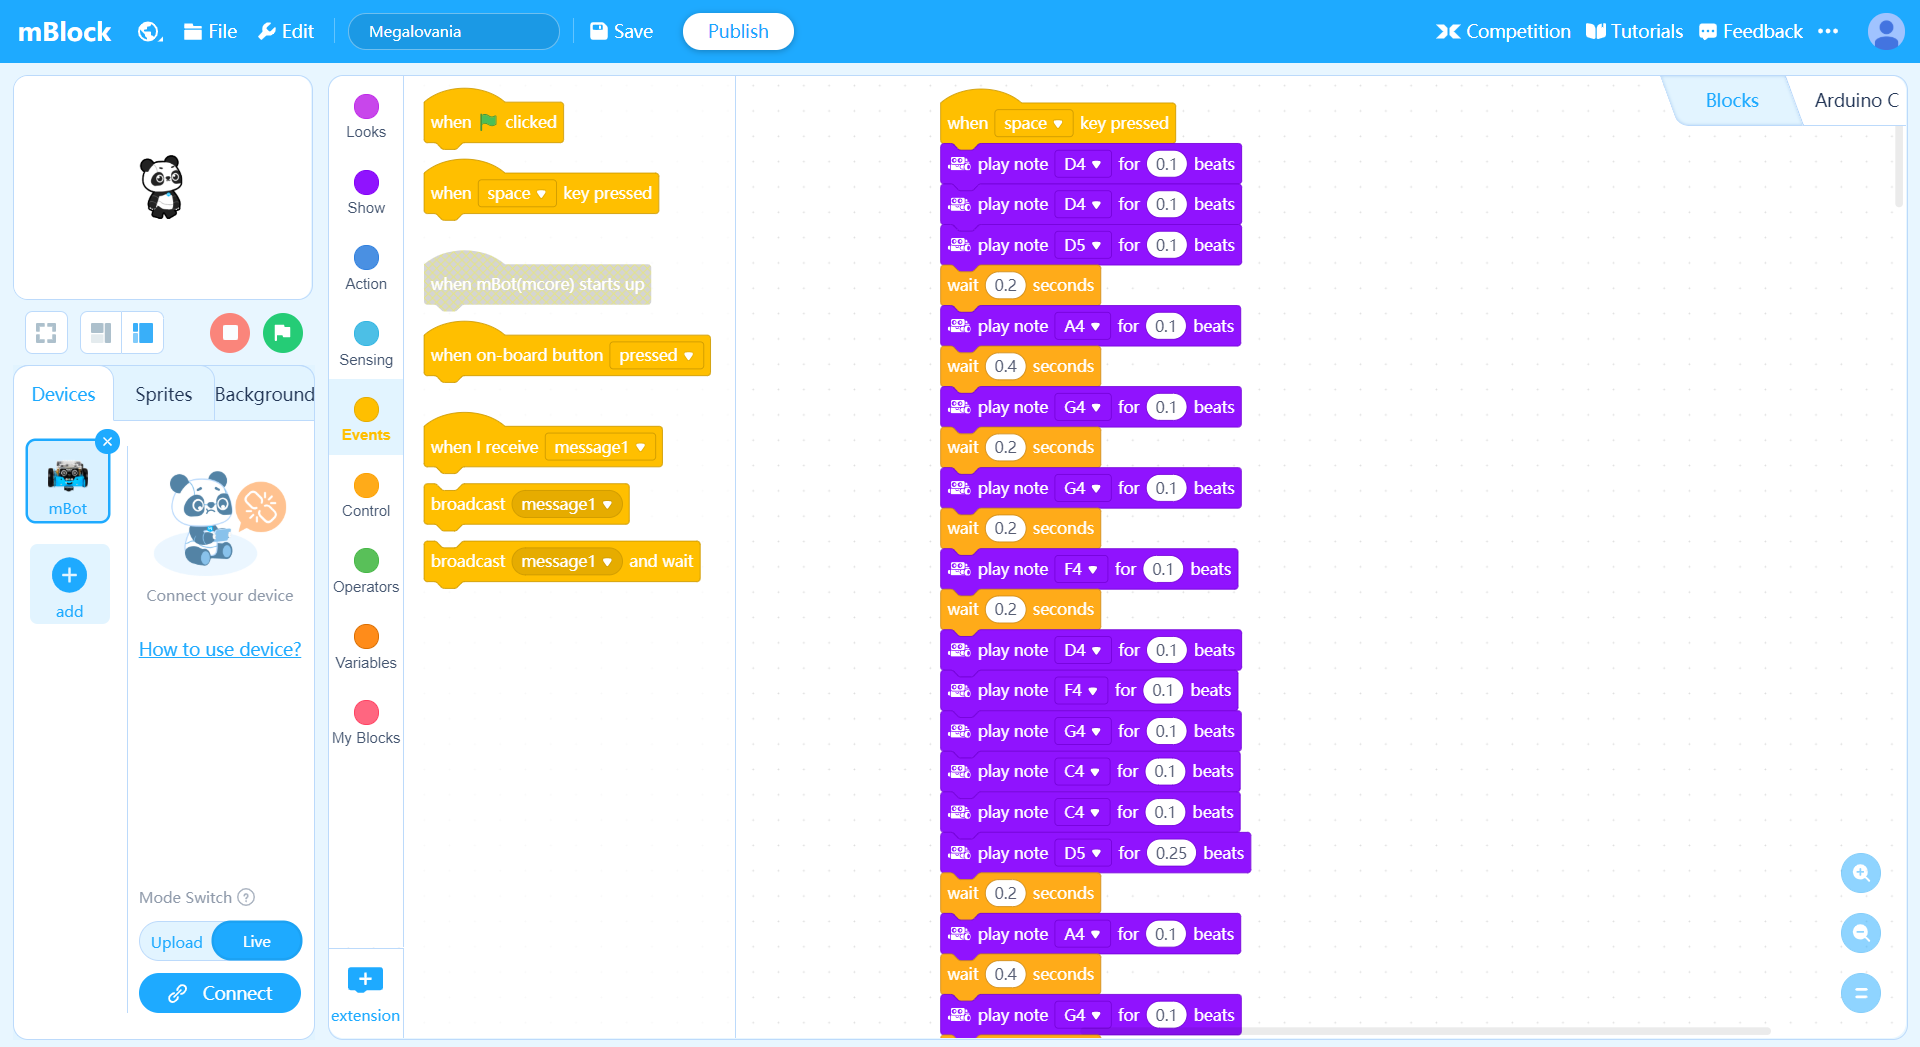
\includegraphics[width=\textwidth]{mblock.PNG}
    \caption{The mBot coding interface, mBlock}
    \label{mblock}
\end{figure}

\section{Critical Analysis}

Before I got this internship, I vaguely knew how regional and departmental councils worked, not knowing what kind of responsibilities and work had to be managed in those. So, when I asked my supervisor to do an internship with him and told him it would be preferable for it to be somewhat related to computer science, and that he responded that he had it covered, I was happily surprised. I didn't know computers and programming were of importance in a departmental council, and nowadays it seems in fact logical for it to gain significance over time, as its uses keep expanding over different domains. As such my supervisor's work is quite relevant towards my studies. Since the Departmental Council is a large administration with a high amount of things to manage, I expected its structure to be vast and complex, spanning multiple branches with each their own smaller intricate structure, and it was exactly this way. One thing I could not correctly theorize about was what task would be given to me. My supervisor is the one responsible for the management of the middle school digital work-space, and as such I first thought my work would have to do with it in one way or another, and in the end, I didn't do anything towards that. He instead decided to give me tasks that weren't that relevant towards his own job but more instructing for me, such as the programming of the mBot. He also gave me some tasks related to his work as that is the point of an internship, like the HTML graph code. And many tasks were also unexpectedly for me not given to me by my supervisor but by his direct superior, who often needed help, preferably my supervisor's, but I was there to take them instead, giving a more diverse range of tasks to do and to learn from. Other than that, the way the Council operates is quite predictable. Every employee has his own tasks to manage, which as an administration, mainly consists of small tasks linked to the management of each one's major task, like the digital work-space for my supervisor, the maintenance and distribution of tablets in the Educational Multimedia Pole, etc. and also contacts through emails or phone calls with different organizations like business firms or people in charge of middle schools for my supervisor. Such is how the Council operates compared to my expectations of it.

\section{SWOT Analysis}

The most important strength of the Departmental Council is its very nature. As stated earlier, since it is a common law community, the Council does not have any competitor. Its role and responsibilities are unique to itself, and because of how the French government works, its existence is a necessity for the department to properly function. This means that it will never disappear unless the departments are revised in which case it might get renamed or merged with another council, but it will never cease to exist. Another strength of the Council is its complex structure. As said in the corresponding section, its structure allows for a high number of responsibilities to be dealt with while having each employee take care of only certain specific tasks. If done correctly this can prove quite beneficial to the organization, however if done wrong this can prove to be also a major weakness. Indeed, the more employees an organization possesses, the more likely it is for one or several of them to do their job incorrectly. It is only natural for people to make mistakes, and sometimes some employees just aren't meant for certain jobs. As such probabilities make this a common weakness amongst organizations. Still, the fact that the responsibilities are more shared keeps being a strength overall even when it might become a weakness, as a mistake made by an employee with few responsibilities will have only little consequences towards the organization. As such the Council suffers from quite common weaknesses that are inevitably found in most organizations, mainly human weaknesses. In terms of opportunities and threats, for the Council, it all comes down to the other organization it interacts with, which depends from what branch of the Council we're looking at. Those organizations are mainly composed of business firms and other organizations under the government that require interaction with the Council to operate. Looking at the Education and Middle Schools Directorate I worked at, I noticed different interactions with other organizations. The first and most obvious kind of organizations were the middle schools the Council has to manage. Because of their relationship with the department, the schools do possess some independence even though most of their management is dealt with by the Council. They can still take part in decision making, project proposing, etc. when it concerns themselves and as such depending on who is in charge, their opinion on certain matters and their efficiency at work, the tasks given to the Directorate can be either easier or harder to accomplish. Most interactions with business firms are done without any problem and anything noteworthy, and sometimes interesting opportunities can come out from such interactions. For instance, most middle schools of the department actually use iPads now, and because of a meeting with Google I had the chance to witness, the Directorate now is trying to operate a switch to Chromebooks, because of how easier to use and more practical for both students and teachers they are compared to iPads, for relatively the same price. Such opportunities come across the various interactions of the Council.

\section{Conclusion}

At the end of the day, the Departmental Council is a regular but important administrative organization. It functions like any other administration, as such it manages most public matters related to the department, makes most decisions concerning those and control in general the evolution of the department. It possesses its own set of strength and weaknesses, which are mostly related to its own nature, and as such mostly cannot be changed in any way. This is obviously both advantageous and unfavorable, but its human weaknesses depend on the employees themselves, and as such are never really the same and are never in the same place or of the same importance. 

\section{Recommendation}

As explained just above, the Council doesn't have a high number of flaws, and as such there is not much to be done. All that can be improved are the employees themselves, and since the perfect employee doesn't exist, same as how a human that doesn't commit any mistake is but a utopia, I cannot make much recommendation for the organization. It is possible that there are flaws I wasn't able to detect during the short time I was working at the Council, thus a deeper analysis of it would be required for a complete understanding of its operation, as well as its strengths and weaknesses.

\section{References \& Sources}

\begin{itemize}
    \item Various information given by my internship supervisor
    \item The official website of the Departmental Council, \textit{valdoise.fr}
    \item Wikipedia pages on common law communities
    \item The official website of french education, \textit{education.gouv.fr}
\end{itemize}

\end{document}
